\chapter{Macchine Astratte}
\section{Macchine Astratte e Linguaggi}
Per analizzare la computabilita' e la complessita' di algoritmi e per implementare nuovi linguaggi di programmazione, risulta necessario avere un modello teorico (realizzato in hardware o software) in grado di eseguire operazioni e memorizzare gli output, che chiamiamo \textbf{macchina astratta}. 

Dare una definizione dettagliata e allo stesso tempo valida per tutti i tipi di macchina astratta e' pressoche' impossibile, dato che esistono molti modelli di computazione che differiscono tra loro, come per esempio il modello logico, funzionale, orientato agli oggetti e altri. Dato che, per motivi puramente tecnologici, la maggior parte delle macchine reali si basano sull'\textbf{architettura di von Neumann}, noi ci soffermeremo sul modello di computazione \textit{imperativo} (le cui caratteristiche essenziali sono strettamente legate a tale architettura).
\subsection{Macchine Astratte Imperative}
\dfn{Macchina Astratta (imperativa)}{
  Una \textbf{macchina astratta (imperativa)} e' un insieme di \textbf{strutture dati} e \textbf{algoritmi} in grado di memorizzare ed eseguire programmi. Le componenti principali sono:
  \begin{itemize}
    \item un \textbf{interprete}
    \item una \textbf{memoria}, contenente sia dati che il programma
    \item un insieme di operazioni primitive
    \item un controllo di sequenza, che ha il compito di acquisire l'istruzione corretta seguendo il flusso dell'algoritmo
    \item un'unita' per il controllo e il trasferimento dei dati in memoria
  \end{itemize}
}
\begin{center}
  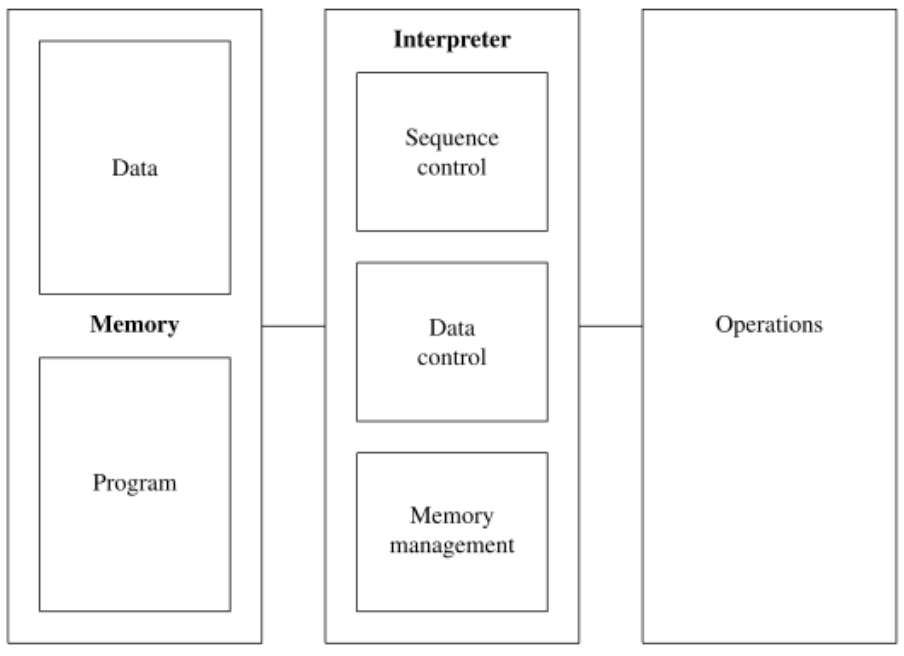
\includegraphics[scale=0.8]{img/AM.png}
  % By M. Gabbrielli and S. Martini - M. Gabbrielli and S. Martini, "Abstract Machines", Undergraduate Topics in Computer Science, pp. 1-25, 2010. Available: 10.1007/978-1-84882-914-5_1., CC BY-SA 4.0, https://commons.wikimedia.org/w/index.php?curid=118069333
\end{center}

\subsubsection{Macchina di von Neumann}
Come accennato prima, l'architettura di von Neumann e' un modello semplice ma estremamente flessibile per la reallizzazione di macchine.

\begin{center}
  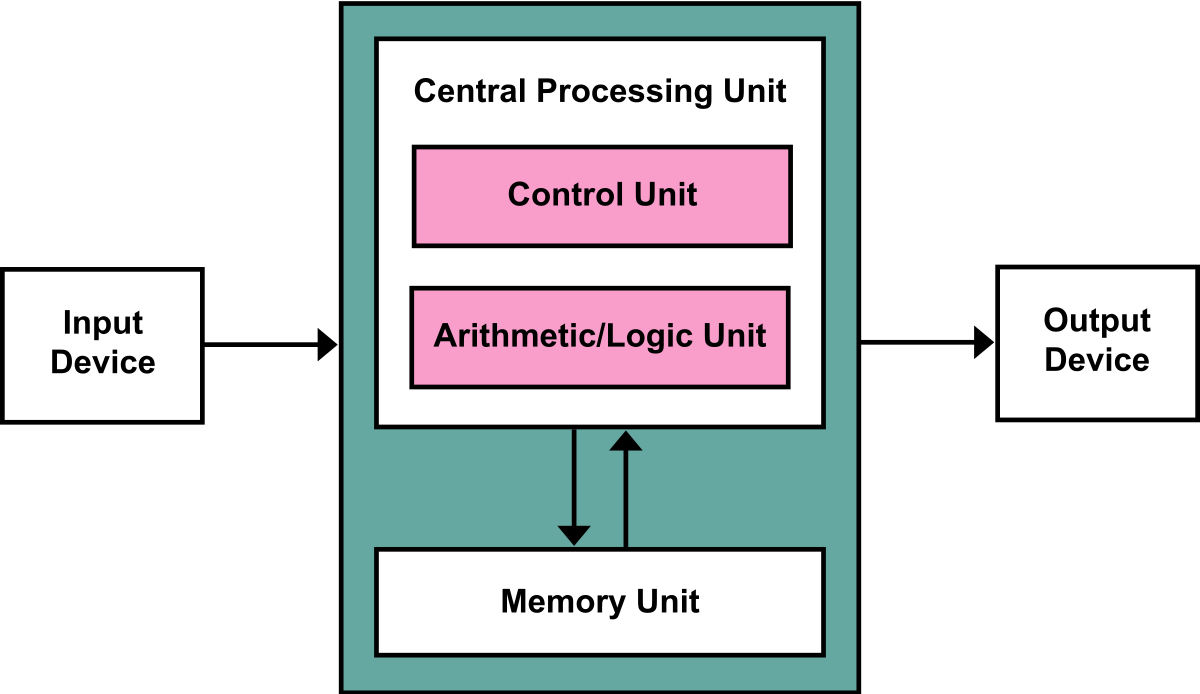
\includegraphics[scale=0.2]{img/VonNeumann.png}
\end{center}

E' un modello ben adatto alla programmazione imperativa, ed e' spesso usata come base concettuale per le macchine astratte imperative. Cio' e' dovuto al concetto di "istruzione" (intrinseca al modello di von Neumann), ovvero operazioni che vengono eseguite in modo sequenziale dall' \textbf{interprete}.

\subsubsection{Interprete}
\label{interp}
L'\textbf{interprete} e' la componente fondamentale che da' alla macchina la capacita' di eseguire programmi. E' un semplice algoritmo, anche chiamato ciclo \textit{fetch-decode-execute}, che permette la corretta esecuzione delle istruzioni, coordinando le componenti della macchina astratta finche' non viene eseguita l'istruzione primitiva di arresto, che provoca l'uscita dal ciclo e l'arresto della macchina

\begin{center}
  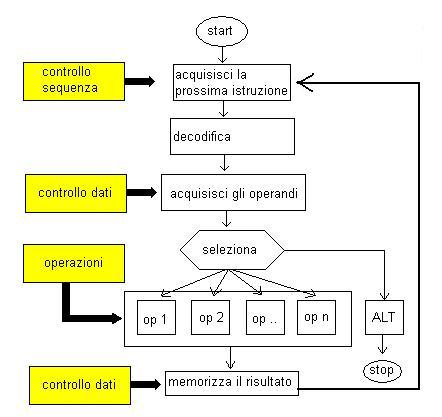
\includegraphics[scale=0.7]{img/Interprete.JPG}
\end{center}

Come si vede dall'immagine, l'interprete e' costituito da operazioni e strutture dati che servono per: (implementazione nelle macchine fisiche)
\begin{itemize}
  \item Elaborare dati primitivi (ALU)
  \item Controllo sequenza di esecuzione (PC e salti)
  \item Controllo dati (Metodi di indirizzamento e trasferimento di blocchi ecc.)
\end{itemize}

La struttura dell'interprete \red{rimane invariata per qualsiasi macchina astratta imperativa}, cambiano le altre componenti.

\subsection{Linguaggio Macchina}
Data una macchina astratta $ M $, chiamiamo $ L_M $ il \textbf{Linguaggio Macchina di M}, ovvero l'insieme delle istruzioni che la macchina $ M $ e' in grado di "comprendere". Per chi programma, il linguaggio che si usa per creare programmi eseguibili da una macchina astratta e' semplicemente una sequenza di caratteri. Mentre all'interno della macchina stessa il programma viene trasformato da algoritmi, che possono sfruttare diverse strutture dati, per diventare un linguaggio comprensibile da una macchina astratta di livello piu' basso, o direttamente dalla macchina fisica (se $ M $ e' realizzata da hardware).

\section{Gerarchie di Macchine Astratte e Linguaggi}
Proviamo a costruire una macchina astratta $ M_\mathcal{L} $ che e' in grado di comprendere ed eseguire istruzioni complesse di un linguaggio $ \mathcal{L} $ di alto livello, partendo da zero. Prima di tutto, vediamo in generale come si forma la gerarchia di macchine astratte:

\subsection{Macchina Hardware}
Per prima cosa dobbiamo per forza partire dal \textbf{livello fisico}, dato che ci serve dell'hardware per eseguire il nostro programma automaticamente. Rimanendo sulla strada di macchine imperative, possiamo utilizzare l'architettura di von Neumann per progettare il sistema. Dobbiamo pero' pensare al linguaggio che l'interprete fisico deve riuscire ad eseguire: teoricamente, sarebbe possibile architettare direttamente un interprete fisico che riesca a comprendere il nostro linguaggio di alto livello, ma questo sarebbe davvero molto costoso e' difficile da implementare, quindi evitiamo. Scegliamo allora una serie di istruzioni basiche, del tipo:
\begin{itemize}
  \item \textbf{Operazioni primitive}: operazioni aritmetico logiche, manipolazione bit, I/O
  \item \textbf{Controllo sequenza}: salti (condizionali), chiamate di subroutine e strutture dati per punti di ritorno di sottoprogrammi
  \item \textbf{Controllo dati}: acquisizione di operandi e memorizzazione dei risultati
    \begin{itemize}
      \item Architettura a registri $ \to $ registri indice e indirizzamento indiretto
      \item Architettura a pila $ \to $ gestione pila
    \end{itemize}
  \item \textbf{Gestione memoria}: 
    \begin{itemize}
      \item Architettura a registri $ \to $ nessuna (memoria statica)
      \item Architettura a pila $ \to $ allocazione e recupero dati sulla pila
    \end{itemize}
\end{itemize}

A seconda del livello di complessita' delle singole istruzioni, possiamo dire che la nostra macchina fisica sia:
\begin{itemize}
  \item \textbf{RISC} (Reduced Instruction Set Computers): istruzioni semplici e solitamente poche
  \item \textbf{CISC} (Complex Instruction Set Computers): istruzioni complesse e solitamente tante
\end{itemize}

L'insieme di queste istruzioni si chiama \textbf{linguaggio macchina}.

\subsection{Macchina Microprogrammata}
A volte, nelle macchine hardware di tipo CISC, e' piu' conveniente creare col \textbf{firmware} una macchina astratta che sta sopra il livello hardware e che interpreti le istruzioni macchina. La \textbf{macchina microprogrammata} traduce queste istruzioni in istruzioni piu' semplici ($ \mu $istruzioni) che puo' eseguire l'interprete della macchina hardware ($ \mu $interprete).

Notare che la macchina microprogrammata deve essere per forza scritta in un linguaggio compreso dal livello inferiore.

\subsection{Macchina Software}
A questo punto possiamo scrivere una macchina astratta utilizzando il linguaggio fornito dalla macchina sottostante. Facciamo cio' per implementare algoritmi e strutture dati piu' complesse, che possono servire anche ai livelli superiori.

Solitamente, dopo il livello hardware (o firmware se c'e'), si trova il livello del Sistema Operativo. La macchina astratta di questo livello e' scritta in linguaggio macchina ed estende le capacita' del livello sottostante implementando primitive di livello piu' alto non presenti al livello hardware (come la gestione file). Tale macchina e' conosciuta come la \textbf{host machine} (macchina ospite o MO).

Partendo dalla macchina ospite possiamo implementare finalmente il nostro linguaggio di alto livello, creando direttamente una macchina astratta che lo riconosce (che sia eseguibile dal Sistema Operativo) o utilizzando una macchina intermediaria, possiamo anche tradurre il linguaggio in uno di livello piu' basso usando un compilatore.

\begin{center}
  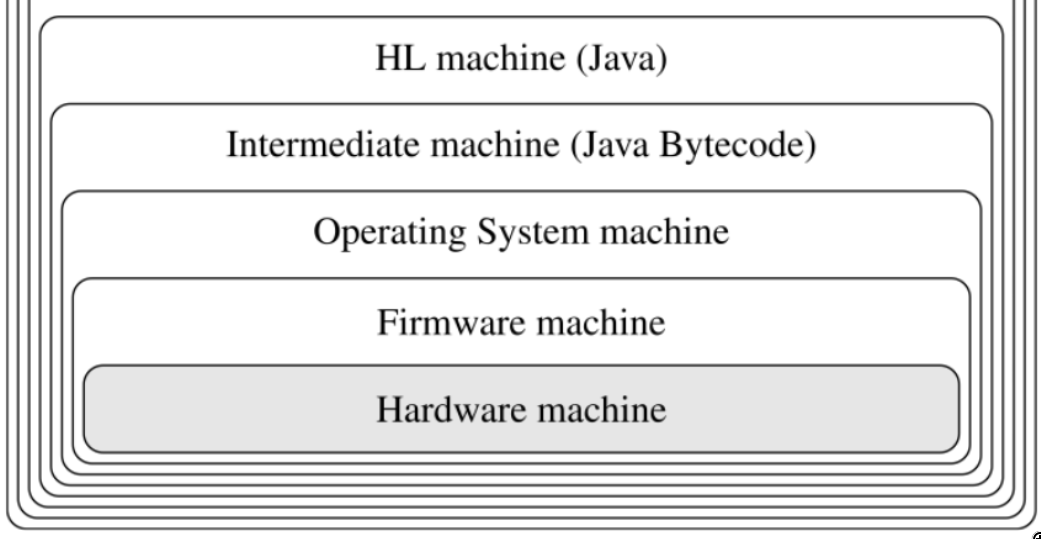
\includegraphics[scale=0.3]{img/2024-12-11-20-16-47.png}
\end{center}

\section{Implementare un linguaggio: Interpreti e Compilatori}
Ora che abbiamo capito come funziona la gerarchia di macchine astratte che ci permette di creare linguaggi di alto livello, definiamo in modo formale il processo:

\subsection{Definizione di programma}
Vogliamo imlementare un linguaggio $ \mathcal{L} $ (cioe' realizzare una macchina astratta $ M_\mathcal{L} $) partendo da una macchina ospite $ M_{\mathcal{L}_O} $. Prima di tutto, definiamo cosa sia un programma scritto in un linguaggio:
\dfn{Programma}{
  $\mathcal{P}_r^\mathcal{L}$ indica un programma $ \mathcal{P}_r $ scritto in un linguaggio $ \mathcal{L} $. 

  A $ \mathcal{P}_r^\mathcal{L} $ e' associata una funzione parziale $ \mathcal{P}^\mathcal{L} $:
  \[
    \mathcal{P}^\mathcal{L}: D \multimap \mspace{-2mu} \to D
  \]
  Dove $ D $ e' l'insieme di dati (se $ \mathcal{P}^\mathcal{L} $ non e' definita per un certo $ d \in D $, allora il programma non termina per quell'input). Tale funzione descrive la \textbf{semantica} del programma $ \mathcal{P}_r^\mathcal{L} $.
}
\nt{
  Per programmi concorrenti la questione e' piu' delicata.
}

Esistono due modi radicalmente diversi per implementare un programma:

\subsection{Implementazione interpretativa pura}
Come abbiamo visto all'inizio del capitolo (\ref{interp}), l'interprete e' la parte fondamentale delle macchine astratte. Quindi, se costruiamo un interprete per un linguaggio $ \mathcal{L} $ usando software scritto con il linguaggio $ \mathcal{L}_O $ della macchina ospite, abbiamo essenzialmente creato una nuova macchina astratta $ M_\mathcal{L} $ sopra a $ M_O $. 

\begin{center}
  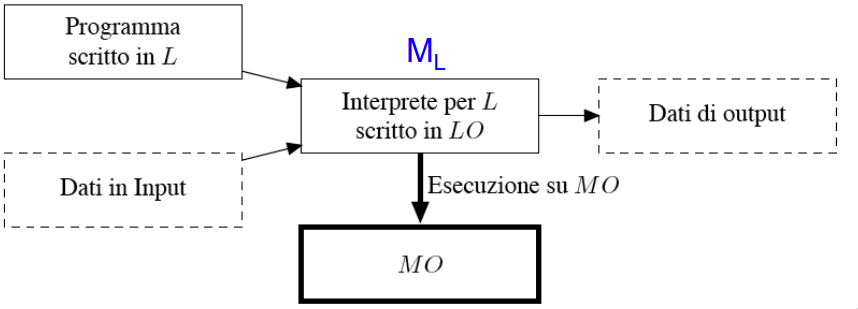
\includegraphics[scale=0.5]{img/2024-12-14-12-08-05.png}
\end{center}

Diamo ora una definizione piu' formale di interprete come funzione (senza interessarci degli aspetti implementativi):
\dfn{Interprete}{
  Un interprete nel lingauggio $ \mathcal{L} $, scritto nel linguaggio $ \mathcal{L}_O $, e' un programma che realizza la funzione parziale:
  \[
    I_\mathcal{L}^{\mathcal{L}_O}: (Prog_\mathcal{L} \times D) \multimap \mspace{-2mu} \to D
  \]
  tale che:
  \[
    I_\mathcal{L}^{\mathcal{L}_O}(\mathcal{P}_r^{\mathcal{L}}, Input) = \mathcal{P}^\mathcal{L}(Input)
  \]
}
Ovvero l'interprete \red{calcola la corretta semantica} del programma scritto nel nostro linguaggio $ \mathcal{L} $.

\subsection{Implementazione compilativa pura}
Oltre all'implementazione interpretativa, esiste un altro modo per rendere un nuovo linguaggio eseguibile su una macchina ospite, che non ha bisogno di creare una nuova macchina astratta (e quindi un nuovo interprete). L'implementazione compilativa si basa sulla \textbf{traduzione} del linguaggio nuovo $ \mathcal{L} $ in un linguaggio riconosciuto da una macchina di livello piu' basso.

\begin{figure*}
  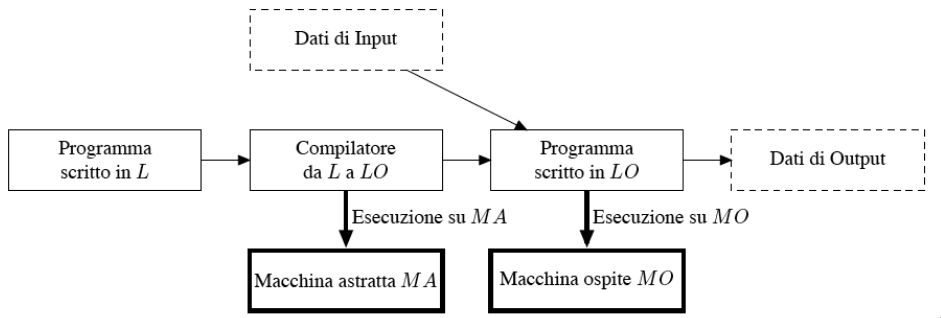
\includegraphics[scale=0.5]{img/2024-12-14-12-09-34.png}
  \caption{Nota: $ M_A $ puo' benissimo coincidere con $ M_O $}
\end{figure*}

Per eseguire tale traduzione, viene usato un programma chiamato \textbf{compilatore}, che puo' essere scritto in un qualunque linguaggio riconosciuto dalle macchine astratte del calcolatore. Il compilatore, quindi, traduce programmi scritti nel linguaggio $ \mathcal{L} $ in nuovi programmi \red{equivalenti} scritti in $ \mathcal{L}_O $:
\dfn{Compilatore}{
  Un compilatore da $ \mathcal{L} $ a $ \mathcal{L}_O $ scritto in un linguaggio $ \mathcal{L}_A $ e' un programma che realizza una funzione:
  \[
    C_{\mathcal{L}, \mathcal{L}_O}^{\mathcal{L}_A}: Prog_\mathcal{L} \to Prog_{\mathcal{L}_O}
  \]
  tale che, dato
  \[
    C_{\mathcal{L}, \mathcal{L}_O}^{\mathcal{L}_A}(P_r^\mathcal{L}) = Pc^{\mathcal{L}_O}_r
  \]
  allora, $ \forall $ Inupt $ \in D $:
  \[
    P^\mathcal{L}(Input) = Pc^{\mathcal{L}_O}_r(Input)
  \]
}
Ovvero il compilatore \red{preserva la semantica} del programma: il programma originale e quello tradotto calcolano la stessa funzione: $ P^\mathcal{L} = Pc^{\mathcal{L}_O} $.

\subsection{Differenze}
Vediamo i pro e i contro dei due metodi:
\begin{itemize}
  \item \textbf{Interprete}
    \begin{center}
      \begin{tabular}{ l | l  }
        Pro & Contro \\
        \hline
        - Flessibile (debugging facile) & - Scarsa efficenza (decodifica per ogni esecuzione) \\
        - Piu' facile da realizzare & \\
        - Occupa meno memoria & 
    \end{tabular}
    \end{center}
  \item \textbf{Compilatore}
    \begin{center}
      \begin{tabular}{ l | l  }
        Pro & Contro \\
        \hline
        - Buona efficenza & - Scarsa flessibilita' \\
        - Piu' facile da realizzare & - Perdita di info (astrazione) del programma sorgente (debuggin difficile) \\
        & - Occupa piu' memoria (non molto rilevante oggi) 
      \end{tabular}
    \end{center}
\end{itemize}

Per riuscire a combinare l'efficenza dei compilatori con la portabilita' dei linguaggi interpretati, nella realta' si utilizza spesso una via di mezzo. Solitamente:
\begin{itemize}
  \item Alcune istruzioni (es. ingresso/uscita) sono sempre \textbf{simulate} (interpretate)
  \item I programmi vengono \textbf{tradotti} in un codice intermedio
\end{itemize}

\begin{center}
  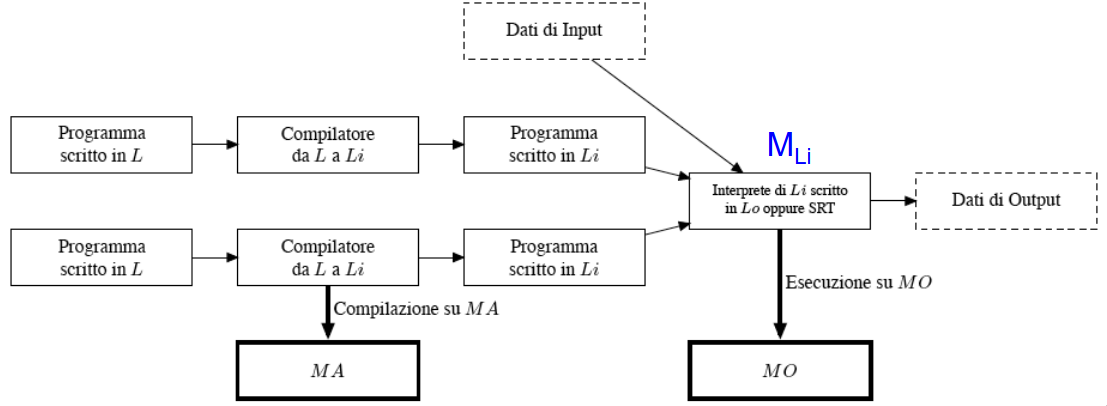
\includegraphics[scale=0.4]{img/2024-12-14-17-02-00.png}
\end{center}

Come si vede nell'immagine, il linguaggio $ L $ viene prima tradotto nel linguaggio intermedio $ L_i $, che poi viene interpretato dall'interprete di $ M_{L_i} $ scritto in $ L_O $. In base a quanto e' diverso l'interprete $ L_i $ da $ L_O $, abbiamo due implementazioni diverse:
\begin{itemize}
  \item Interpretativa: l'interprete della macchina intermedia $ M_{L_i} $ e' sostanzialmente diverso dall'interprete della macchina ospite $ M_{L_O} $. (Es. Java)
  \item Compilativa: $ M_{L_i} = M_{L_O} +  $ opportuni meccanismi, come I/O, gestione memoria, ecc. (Es. C)
\end{itemize}

\subsubsection{Cosa interpretare e cosa compilare}

Abbiamo visto che le soluzioni di tipo compilative sono piu' effcenti, mentre quelle di tipo interpretativo privilegiano flessibilita' e portabilita'. In linea di principio:
\begin{itemize}
  \item Traduzione per i costrutti di $ L $ che corrispondono da vicino a costrutti di $ L_O $
  \item Simulazione per gli altri
\end{itemize}

\subsection{Generazione Compilatori}

Ora che abbiamo esplorato i modi per eseguire programmi scritti in un linguaggio nuovo usando compilatori e interpreti, vediamo come costruire questi ultimi strumenti.

\subsubsection{Si possono sempre realizzare?}
Immaginiamo un interprete e un compilatore scritti nello stesso linguaggio $ L_{osp} $ e che ricevono in input lo stesso linguaggio $ L_{sorg} $. L'interprete e' in grado di calcolare la semantica del programma in input usando $ L_{osp} $ e il compilatore preserva la semantica del programma tradotto, quindi tutte le funzioni che $ L_{sorg} $ puo' calcolare possono essere simulate o tradotte con $ L_{osp} $. Quindi:
\[
L_{osp} \text{ e' non meno espressivo di } L_{sorg}
\]
Dato che, come vedremo piu' avanti, tutti i linguaggi di programmazione "veri" \red{sequenziali} sono ugualmente espressivi (Turing-completi, se forniti di memoria "illimitata"), allora sappiamo che questa condizione vale sempre (se $ L_{osp} $ e' un "vero" linguaggi sequenziale).

\nt{
  Esistono formalismi/linguaggi molto meno espressivi ma che sono utilissimi per la loro efficenza, come ad esempio:
  \begin{itemize}
    \item Automi finiti (analizzatori lessicali)
    \item Automi a pila (analizzatori sintattici)
  \end{itemize}
}

\subsubsection{Come viene generato un compilatore?}

Esistono diversi modi per creare un compilatore/interprete dato un linguaggio $ L $:
\begin{itemize}
  \item \textbf{Strumenti automatici}
    \begin{itemize}
      \item \textbf{Lex}: generatore di analizzatori \textbf{lessicali}
      \item \textbf{Yacc}: generatore di analizzatori \textbf{sintattici}
    \end{itemize}
    Data una descrizione formale della sintassi di $ L $, questi strumenti sono in grado di generare automaticamente un programma che riesce a riconoscere stringhe sintatticamente legali.
  \item \textbf{Implementazione via Kernel}

    Si sceglie $ H \subset L $, ovvero un sottoinisieme proprio di $ L $ che forma un nucleo (kernel) con il quale possiamo costruire:
    \begin{itemize}
      \item $ C^H_{L, L_O} $, ovvero un compilatore scritto in $ H $ che traduce $ L $ in $ L_O $, oppure
      \item $ I^H_L $, ovvero un interprete per $ L $ scritto in $ H $
    \end{itemize}
    Manca poi scrivere un interprete/compilatore per $ H $, in modo da poter eseguire uno di questi due sulla macchina ospite, che se $ H $ e' stato scelto bene non dovrebbe essere troppo difficile.

    Implementare prima un sottoinsieme di $ L $ porta a dei vantaggi:
    \begin{itemize}
      \item Semplifica l'implementazione, dato che $ H $ e' piu' vicina a $ L $ rispetto a $ L_O $
      \item Facilita la portabilita, perche' basta re-implementare $ H $ nel nuovo linguaggio macchina
    \end{itemize}
  \item \textbf{Bootstrapping}

    Immaginiamo di aver creato i seguenti compilatori e interprete, dove $ M_i $ e' una macchina astratta intermedia:
    \begin{itemize}
      \item $ C^{L_i}_{L, L_i} $
      \item $ I^{L_O}_{L_i} $
      \item $ C^L_{L, L_O} $
    \end{itemize}
    Otteniamo un compilatore per $ L $ scritto in $ L_O $ in questo modo:
    \[
      I^{L_O}_{L_i}(C^{L_i}_{L, L_i}, C^L_{L, L_O}) = C^{L_i}_{L, L_O}
    \]
    \[
      I^{L_O}_{L_i}(C^{L_i}_{L, L_O}, C^L_{L, L_O}) = C^{L_O}_{L, L_O}
    \]
    Piu' efficente rispetto al kernel, dato che abbiamo un compilatore che compila direttamente al linguaggio di $ M_O $ senza usare un linguaggio intermedio.

\end{itemize}
